%% Settings for single-side (simplex) printing
% Margins: left 40mm, right 25mm, top and bottom 25mm
% (but beware, LaTeX adds 1in implicitly)
\documentclass[12pt,a4paper]{report}
\setlength\textwidth{160mm}

\usepackage[utf8]{inputenc}
\usepackage{graphicx}
\usepackage{fancyhdr}
\usepackage{lmodern}
\usepackage{lastpage}
\usepackage{subfig}
\usepackage{hyperref}

\graphicspath{{../graphs/}}

\pagestyle{fancy}
\fancyhf{}
\rhead{Petr Houška `houskape@gmail.com`}
\lhead{HW3: Matrix transposition}
\rfoot{Page \thepage / \pageref{LastPage}}


\begin{document}
	
	\section{Reálné CPU}
	\begin{figure}[h]	
		\centering	
		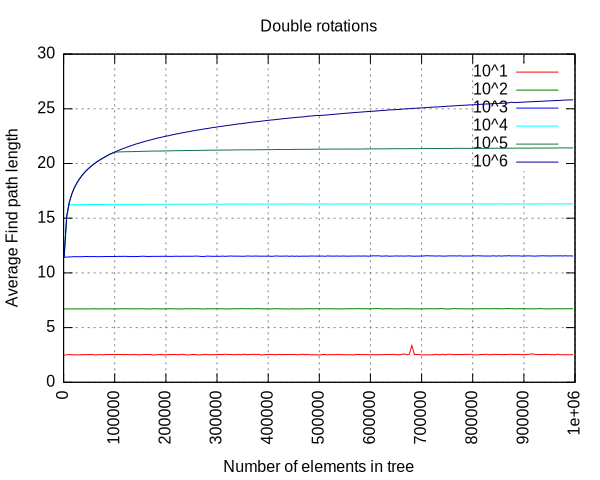
\includegraphics[scale=0.6]{graph_1}		
	\end{figure}

	Na prvním grafu vidíme porovnání průměrného času na prohození dvou prvků pro naivní algoritmus a rekurzivní cache oblivious algoritmus, který se zastaví na podmatici velikosti 8x8 a dál pokračuje naivně. 
	
	\subsection{Cache oblivious}
	
	Pro cache oblivious algoritmus jsou zřejmé dva segmenty, s rozhraním okolo cirka $800^2$ prvků. Skok mezi těmito dvěma segmenty není nikterak výrazný, z $1.5 * 10^{-6}$ na $4.0 * 10^{-6}$.
	
	Tento skok přibližně odpovídá tomu, kdy se celá matice ($640 000$ prvků, 3MB) ještě vleze do L3 cache. Skok tedy začíná trochu dříve než by čistě matematicky měl. I pro $n == 1000$ (4MB) by se do L3 matice měla vejít celá, nicméně kvůli asociativitě cache a komplikovanosti dnešního HW není úplně překvapivé, že ke zhoršování průměrného času dochází před úplným naplněním.
	
	Byť to z grafu není úplně vidět, tak čistá data naznačují, že podobný skok by mohl být i u hranice velikosti L2 a L3 cache. Konkrétně pro $n \approx 256$, kdy se celá matice ještě vejde do L2, se průměrný čas přístupu zvedne z $1.2 * 10^{-6}$ na $1.4 * 10^{-6}$. Kvůli šumu a skokům k vyšším hodnotám pro určitá $n$ (téměř jistě kvůli asociativitě) se ovšem nedá říct nic s jistotou. 
	
	Na rozhraní $n$ pro matice, které se těsně vejdou do L1 cache žádný pozorovatelný rozdíl není. 
			
	\subsection{Naive}
	U naivního algoritmu jsou jasně pozorovatelné segmenty 3. Od začátku do $1000^2$ prvků, kde se průměrný čas pohybuje okolo $1.5 * 10^{-6}$, tedy stejně jako u cache oblivious algoritmu. Následně do 	$20 000^2$ prvků, kdy je čas okolo $1-2 * 10^{-5}$, a nakonec poslední segment, ve kterém čas roste až k $5*10^{-5}$ milisekund na prohození.
	
	
	První skok odpovídá již dříve popsanému přechodu z toho, kdy se celá matice ještě vleze do L3 cache a kdy už ne. Dokud se vleze, tak je naivní algoritmus, s výjimkou $n == 512$, naprosto srovnatelný s cache aware variantou. Pro $n == 512$ se téměř určitě projevuje asociativita cache. Ta má která má, vzhledem k access patternu, daleko větší dopad v případě naivního přístupu (kde přistupujeme postupě na všechny řádky pod sebou, které jsou od sebe přesně o $4*512$B) než v případě cache oblivious.
	
	To že je naivní přístup až do $n$, kdy se matice nevejde do L3 cache, srovnatelný s cache oblivious algoritmem jen dále podporuje tezi, že mezi tím, jestli se matice vejde do L1, L2 nebo jen L3 není žádný významně pozorovatelný rozdíl, který by nebyl z větší části vynahrazen cache pre-fetchem a zamaskován ostatními vlivy. Pokud by totiž přesouvání z L3 cache do L1 a L2 mělo výrazný overhead, tak by se tento overhead nutně více projevil v naivním algoritmu (cache oblivious přístup tyto přesuny minimalizuje).
	
	Od $n$, kdy se matice už nevleze do L3 cache roste průměrná doba swapu postupně až do $n \approx 22 000$ (matice velikosti 2GB), kdy začne raketově růst z $2 * 10^{-5}$ k $5 * 10^{-5}$ milisekundám. Tam se následně, byť v velkým rozptylem, drží až do maximální testované velikostí $n == 44591$ (7.9 GB).
	
	Tento růst a obecně velký rozptyl v druhém i třetím segmentu si vysvětlují tím, jak je paměť RAM strukturovaná. Za zmínku stojí ještě vyšší průměrný čas vždy když je $n$ násobkem mocin $2$. Z části to bude způsobené tím, že u poloviny přístupů (ty co jdou v rámci řádku) se bude více projevovat cache aliasing (viz výše) způsobený asociativností cache. Z části to může být způsobené také strukturou paměti RAM, nicméně na posouzení toho co má konkrétně jaký vliv nemám dostatečné znalosti.
	
	\section{Simulátor}
	\begin{figure}[h]	
	\centering	
	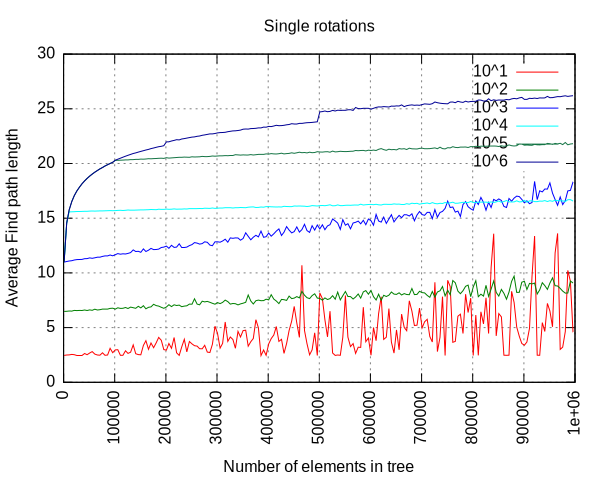
\includegraphics[scale=0.6]{graph_2}		
	\end{figure}

	Na grafu ze simulátoru jsou 

	\begin{figure}[h]	
    \centering
		\subfloat{{\includegraphics[scale=0.4]{graph_2_adv}}}%
		\qquad
		\subfloat{{\includegraphics[scale=0.4]{graph_2_naive}}}%
    \end{figure}




\end{document}